\chapter{Présentation Générale}



\section{Archétype}

L'objectif est de réaliser un jeu video de type Tactical RPG dans l'idée du jeu Disgaea.


\begin{figure}[H]
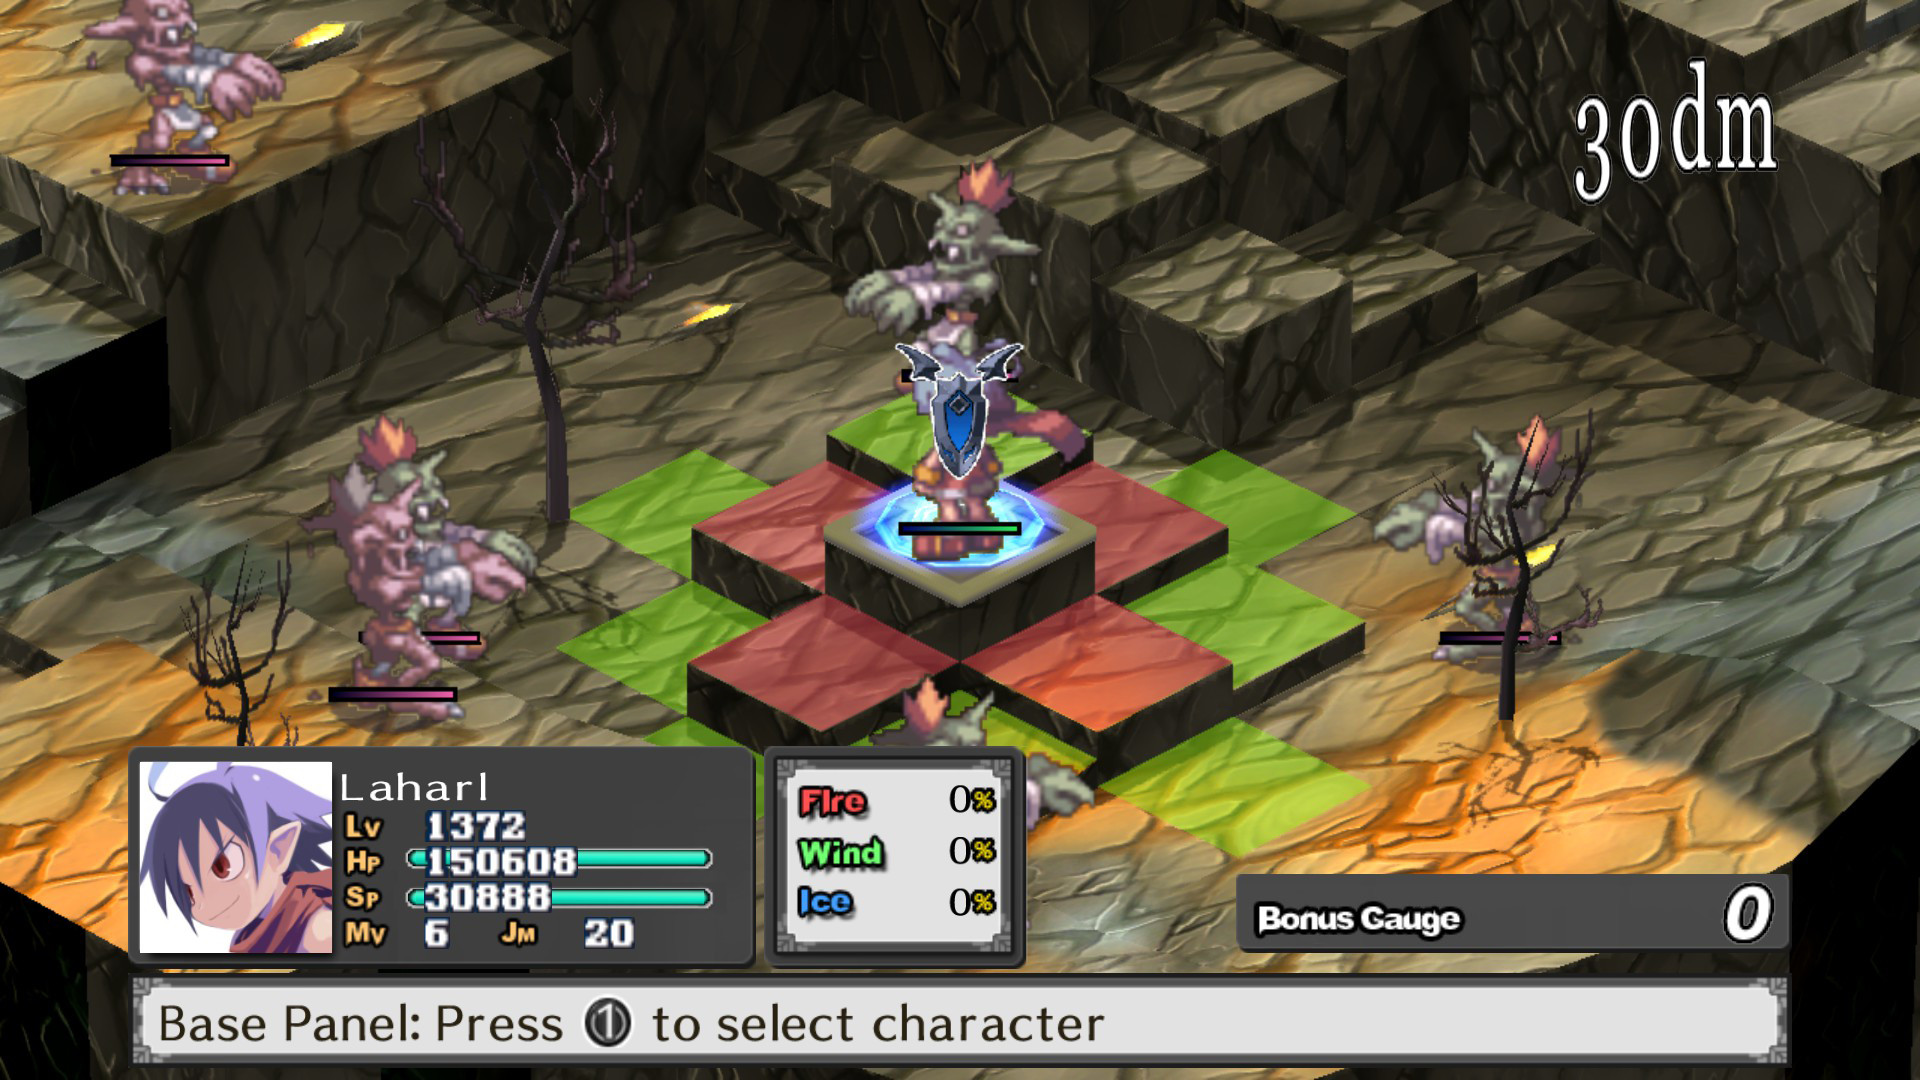
\includegraphics[width=\linewidth]{images/disgaea_exemple.png}
\centering
\caption{Aperçu de l'ecran de Jeu du jeu Disgaea}
\label{fig:img1}
\end{figure}



\section{Règles du Jeu}


\subsection{But du Jeu}
Les joueurs ont chacun un nombre défini de troupes positionné sur la carte.
Le But du jeu est d'éliminer l'ensemble des troupes ennemies (condition de victoire).
Ou d'avoir toutes ses troupes éliminées (condition de défaite).
\\
Une unité est considérée comme détruire lorsque ses points de vie tombent à 0.

\subsection{Tour de Jeu}
Le jeu se découpe en une sucession de tours. Les joueurs jouent les uns à la suite des autres.

Dans un tour, le joueur peut: \\

\begin{itemize}
  \item Déplacer ses unités sur la carte sur un nombre limité de cases.
  \item Attaquer avec ses unités des unités adverses adjacentes ou à distance en fonction du type d'attaque utilisable par l'unité. 
  \item Appliquer une posture de défense sur ses unités pour augmenter la défense si attaquée. 
  \item Utiliser des objets sur ses unités pour la soigner etc...

\end{itemize}

\subsection{Terrain de Jeu}

Le terrain est décomposé en tuiles. Une unité reçoit des bonus ou des malus en fonction de la tuile sur laquelle elle se trouve. Une unité placée sur une tuile de forêt par exemple recevra un bonus d'esquive si attaquée.\\

Les tuiles peuvent avoir des hauteurs différentes. Une unité placée sur une tuile en hauteur aura une meilleure portée pour des attaques à distance, mais y accèder coûte plus de points de déplacement.

\section{Ressources}

\begin{figure}[H]
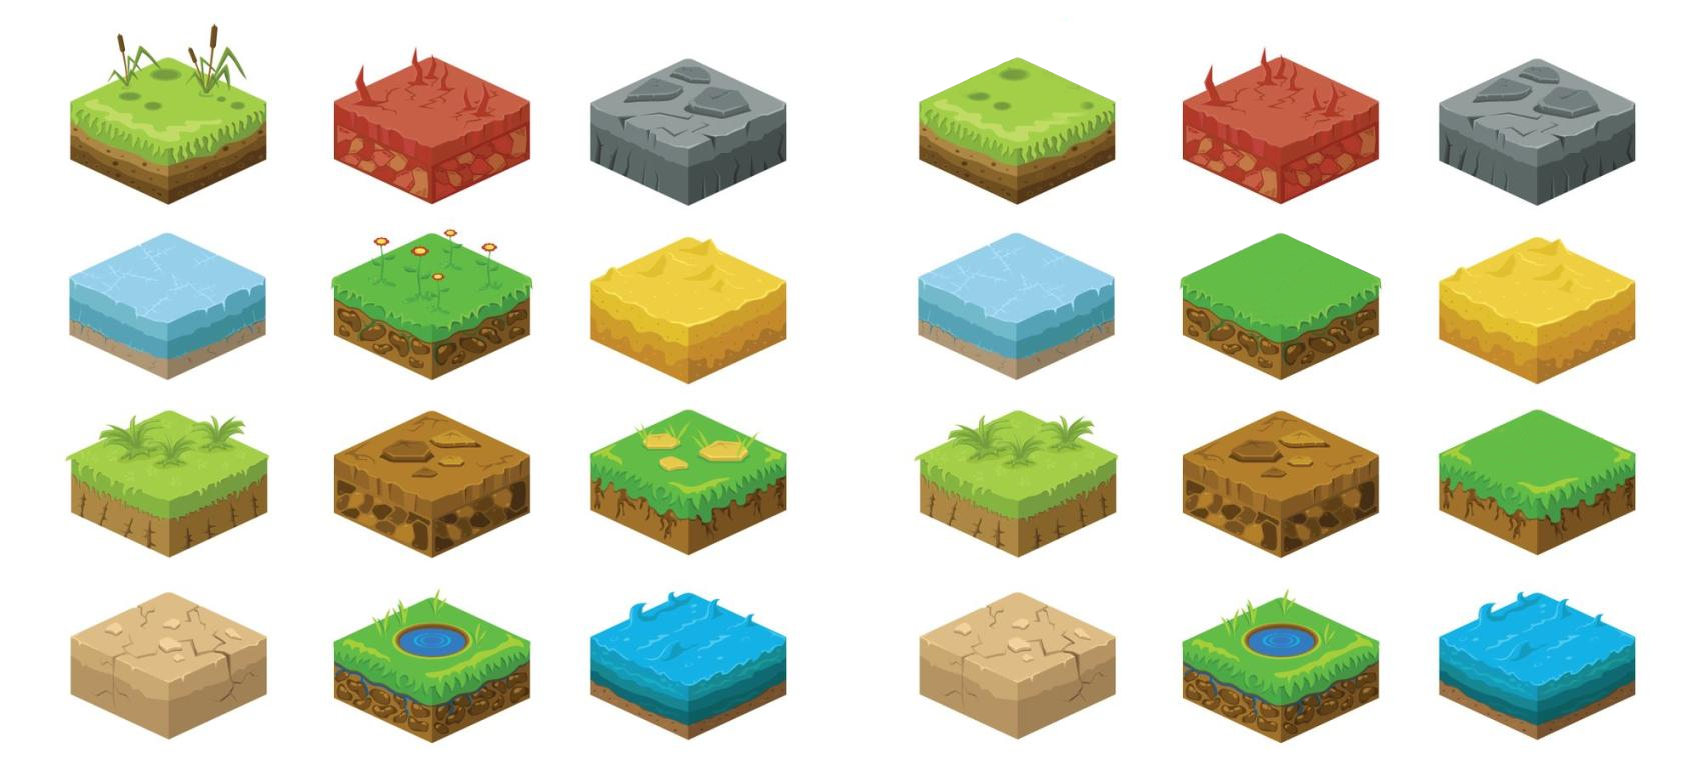
\includegraphics[width=\linewidth]{images/maptiles.png}
\centering
\caption{Tiles pour la carte en perspective isométrique}
\label{fig:img2}
\end{figure}

\begin{figure}[H]
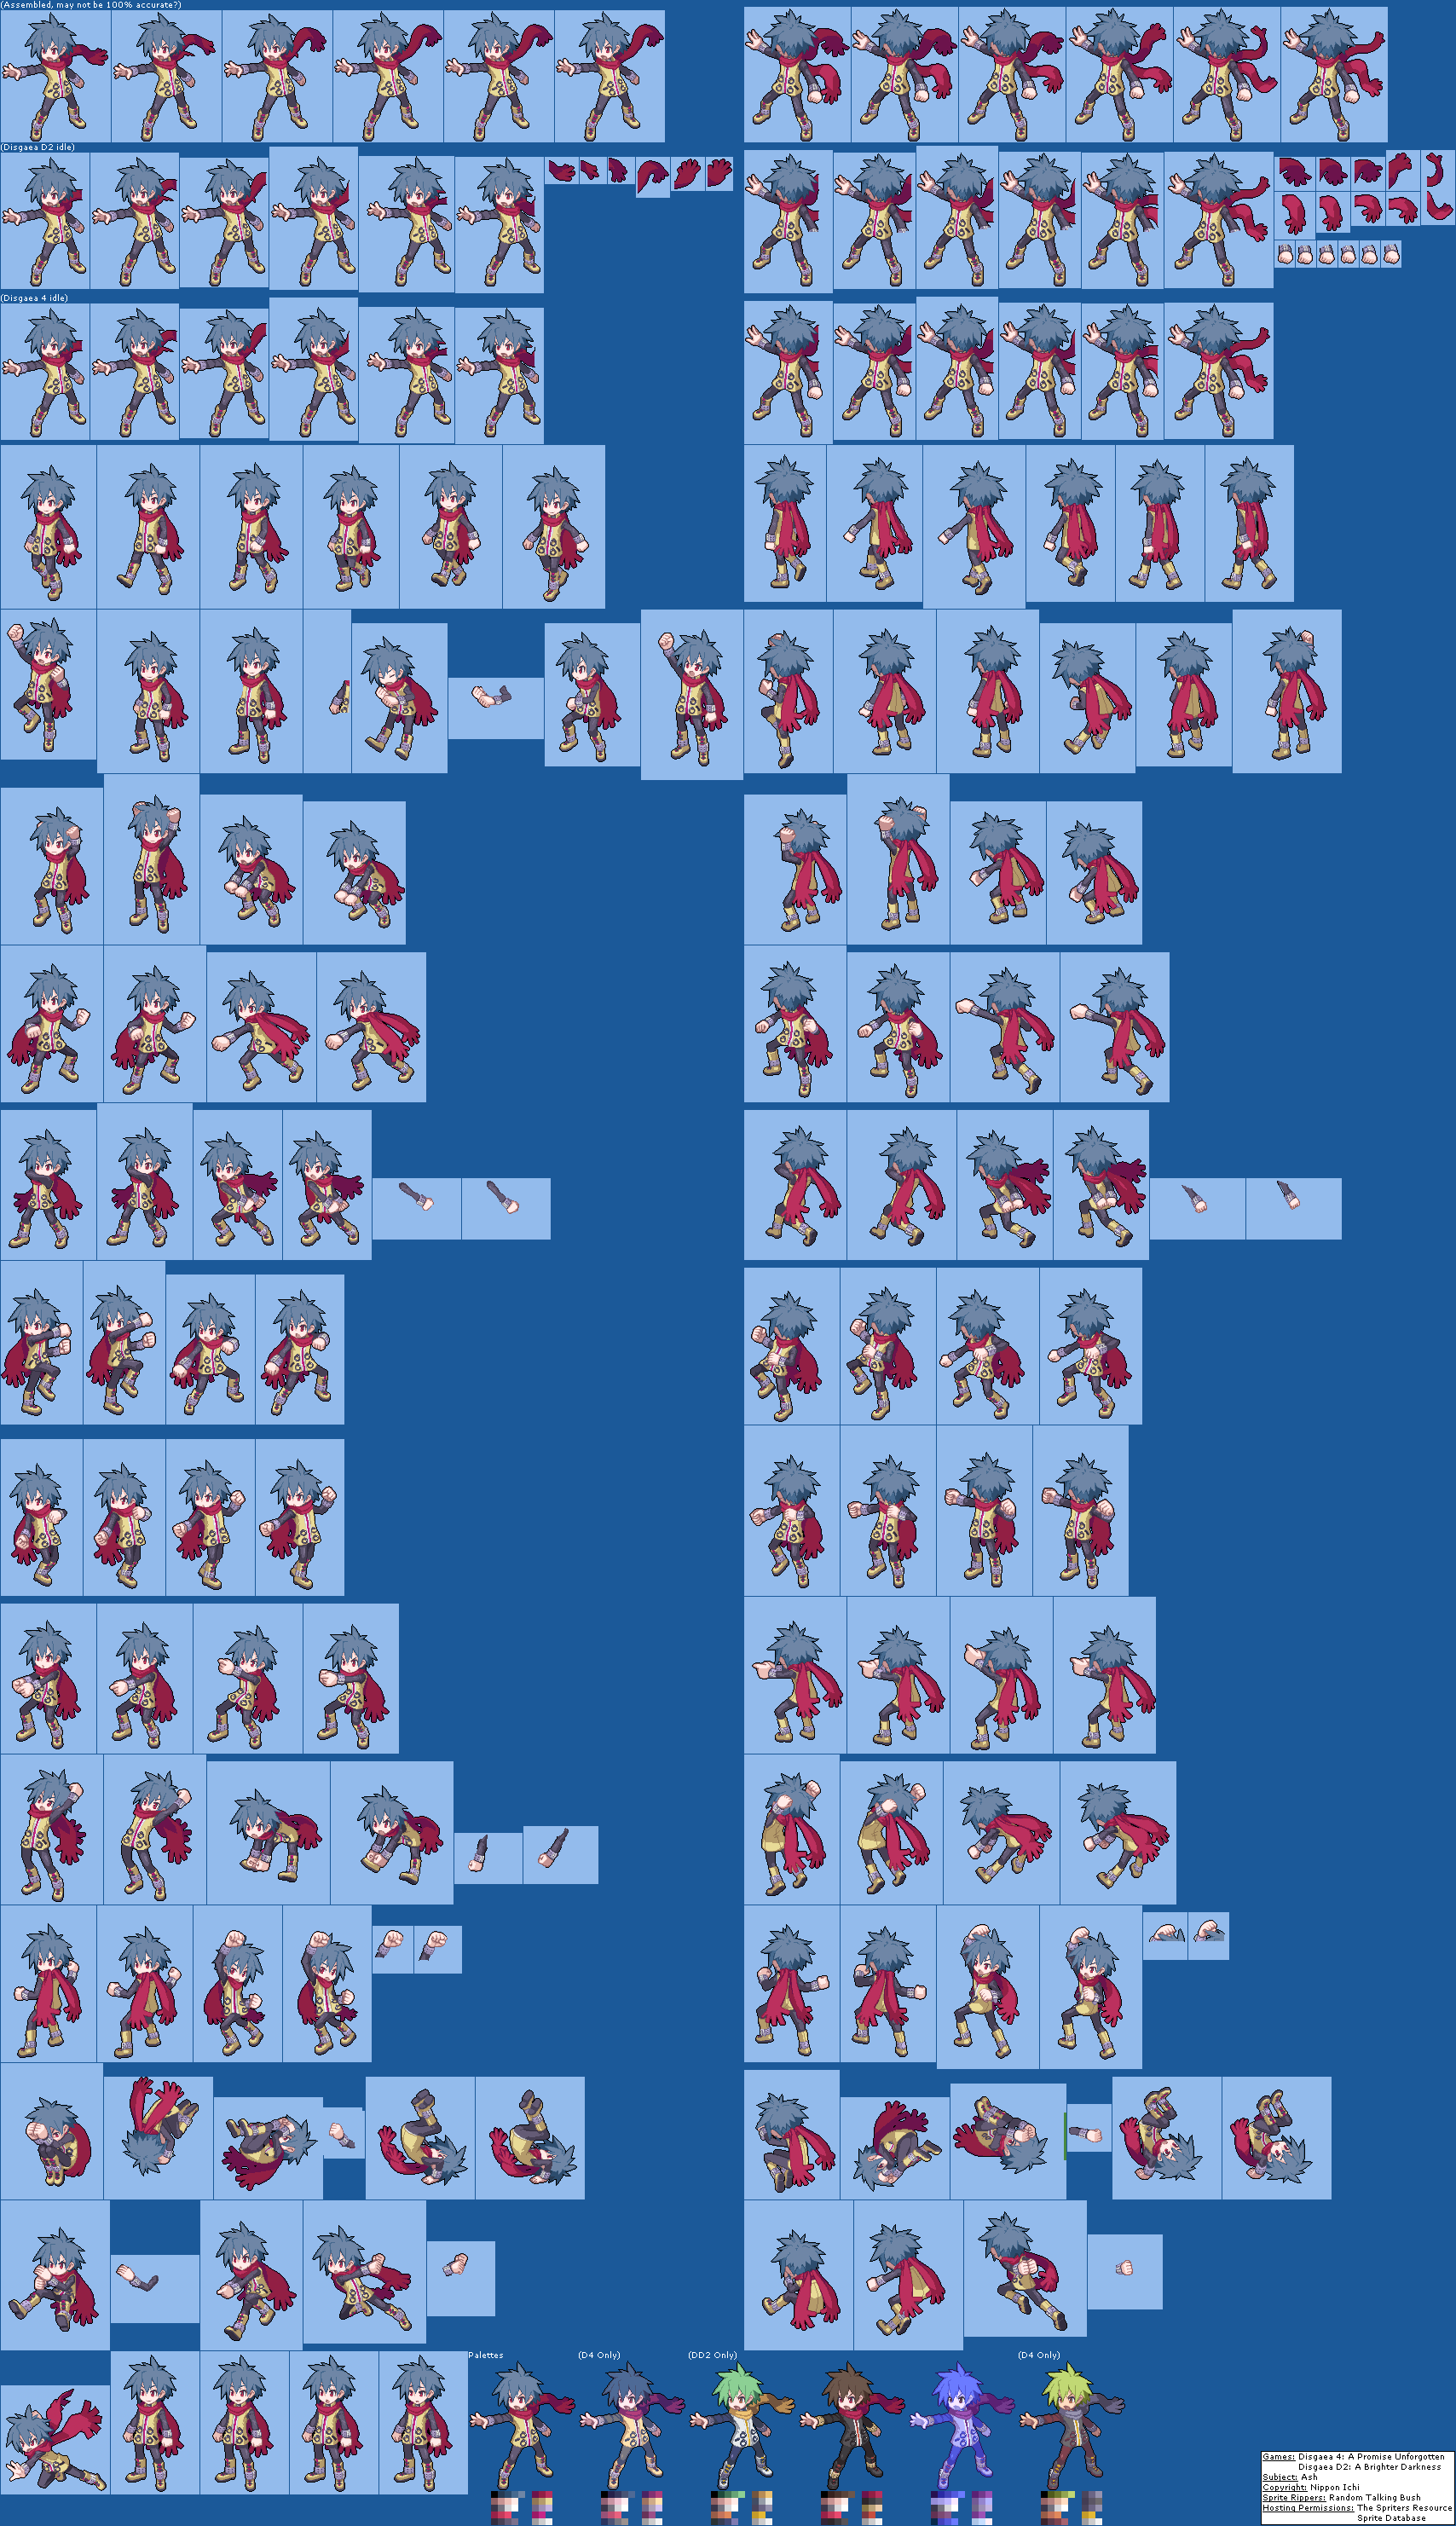
\includegraphics[scale=0.15]{images/char1.png}
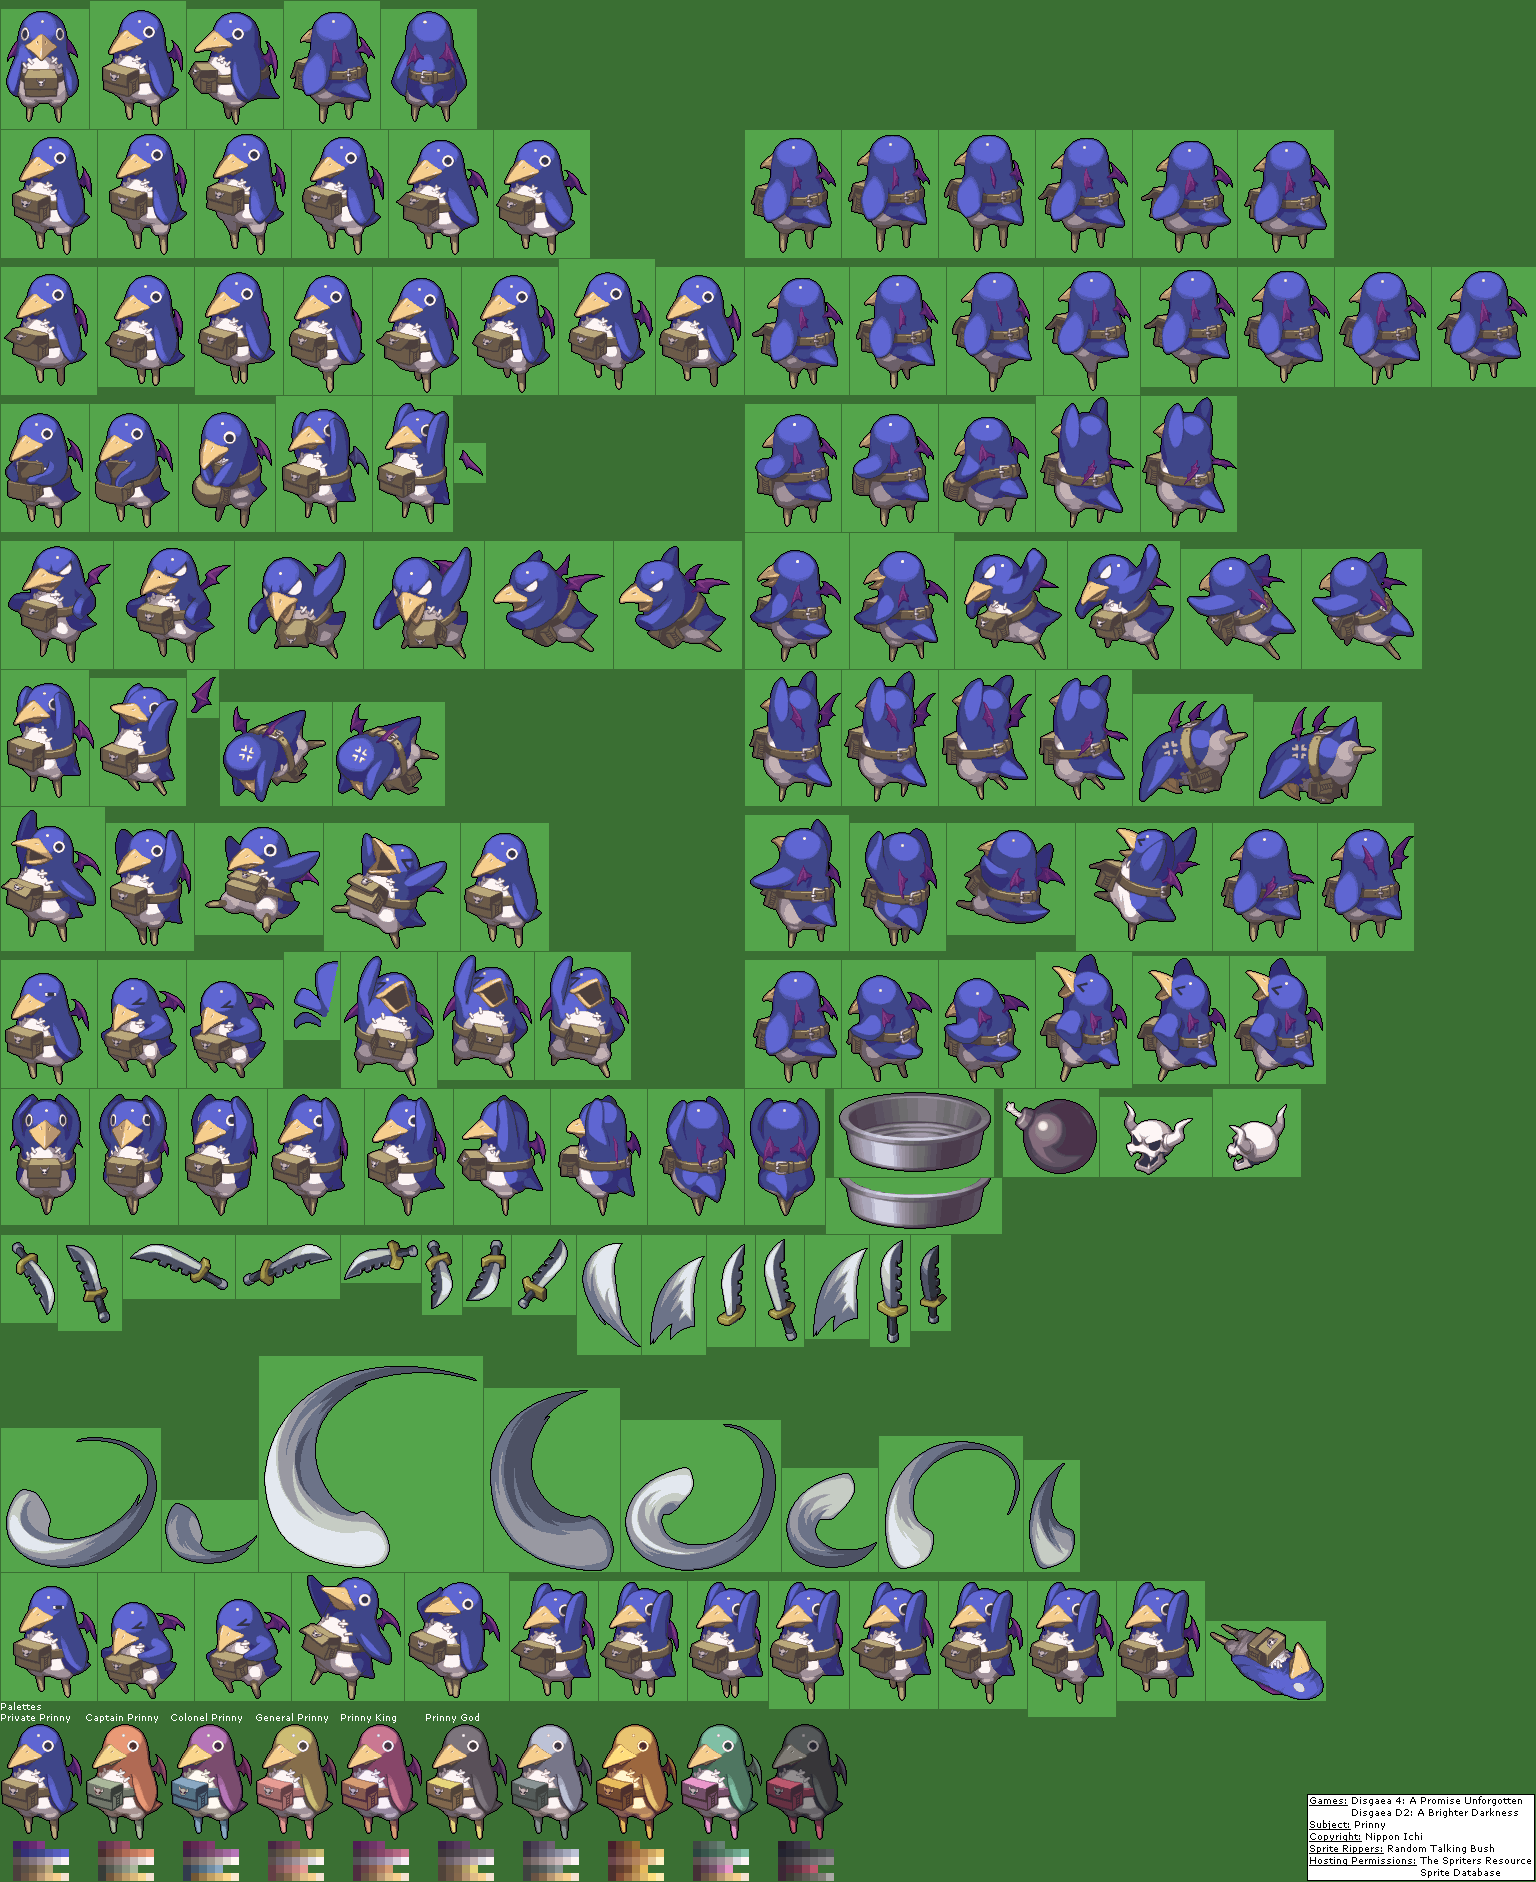
\includegraphics[scale=0.15]{images/enn1.png}
\centering
\caption{Spritesheets personnages}
\label{fig:img3}
\end{figure}
